\documentclass[11pt]{amsart}
\usepackage{geometry}                % See geometry.pdf to learn the layout options. There are lots.
\geometry{letterpaper}                   % ... or a4paper or a5paper or ...
%\geometry{landscape}                % Activate for for rotated page geometry
%\usepackage[parfill]{parskip}    % Activate to begin paragraphs with an empty line rather than an indent
\usepackage{graphicx}
\usepackage{diagbox}
\usepackage{amssymb}
\usepackage{xcolor}
\usepackage{epstopdf}
\usepackage{float}
\usepackage[font={footnotesize}]{caption}
\usepackage{slashbox}
\usepackage{amsmath,amsfonts,amsthm,url,array,etoolbox}
\usepackage{enumerate}
\usepackage{tikz}
\usepackage{pgfplots}
\usepackage[titlenumbered,ruled]{algorithm2e}
\usetikzlibrary{arrows,positioning,calc,decorations.markings}
\theoremstyle{plain}
%\usepackage{titlesec}

\setcounter{secnumdepth}{4}

%\titleformat{\paragraph}
%{\normalfont\normalsize\bfseries}{\theparagraph}{1em}{}
%\titlespacing*{\paragraph}
%{0pt}{3.25ex plus 1ex minus .2ex}{1.5ex plus .2ex}

\newtheorem{thm}{Theorem}
\newtheorem{lem}[thm]{Lemma}
\newtheorem{prop}[thm]{Proposition}
\newtheorem{cor}{Corollary}

\theoremstyle{definition}
\newtheorem{defn}{Definition}
\newtheorem{conj}{Conjecture}
\newtheorem*{exmp*}{Example}%%no label here.

\theoremstyle{remark}
\newtheorem{rem}{Remark}
\newtheorem*{note}{Note}
\DeclareGraphicsRule{.tif}{png}{.png}{`convert #1 `dirname #1`/`basename #1 .tif`.png}

\tikzset{
    %Define standard arrow tip
    >=stealth',
    % Define arrow style
    pil/.style={
           ->,
           thick}
}
\begin{document}


\title[geXGB]{A gene-based exchanged XGBoost method for detecting and ranking gene-gene interactions of qualitative trait}


\author{Yingjie GUO}

\author{Chenxi WU}
\address{Chenxi Wu, Max Planck Institute for Mathematics, Vivatsgasse 7 Bonn, Germany}
\email{wuchenxi2013@gmail.com}

\author{Ao LI}

\author{Xiaoyan LIU}

\author{Junwei ZHANG}

\author{Alon KEINAN}

\author{Maozu GUO}

\maketitle


\begin{abstract}
Among the large of number of statistical methods that have been proposed to identify gene-gene interaction in case-control genome-wide association studies (GWAS), gene-based methods have recently grown in popularity as they confer advantage in both statistical power and biological interpretability.
All of the gene-based methods either jointly model the distribution of single nucleotide polymorphism (SNPs) sets prior to the statistical test, or specify an explicit function form of traits and SNPs, leading to a limited power to detect XXX.
In this paper, we instead proposed a gene-based method that first applies XGBoost, a popular and highly effective boosted tree methods in machine learning for modeling additive models with non-linear terms, to model the function of qualitative trait with all the genes to be considered, and then form a subsample with an exchange strategy to evaluate the interaction of each pair of genes as a deviation from the multiplicative structure in the predicted probabilities.
We use simulations to assess the capacity of geXGB. The benefits of our approach in terms of statistical power and robustness of genes are evaluated in pure and strict disease models with a wide range of heritability and MAF by comparing it to previous methods. We also apply our method to the gene pairs associated to rheumatoid arthritis(RA)in the Wellcome Trust Case Control Consortium(WTCCC)dataset according to the RA pathway hsa05323 in KEGG.
\end{abstract}

%\section{Introduction}

Genome-wide association studies (GWAS) are a well-established and effective method of identifying genetic loci associated with common diseases or traits and have identified over twenty-four thousand unique single-nucleotide polymorphisms-trait (SNPs) associations \cite{21,22}. Earlier GWAS analysis strategies were largely based on single locus models, which test the association between individual markers and a given phenotype independently. Although this type of approaches have successfully identified many regions of disease susceptibility, most of these SNPs identified have small effect sizes which failed to fully account for the heritability of complex traits. Genetic interaction has been hypothesized to play an important role in the genetic basis of complex diseases and traits\cite{23,24,25} and to be one of the possible solutions to this problem of ``missing heritability''\cite{26,27,28}. Even if genetic interaction explains only a tiny fraction of ``missing heritability'', they can still provide some biological insight on the pathway level through by aiding the construction of novel gene pathway topologies.\\

\noindent The first investigations on genetic interactions have been at the SNP level, in which various statistical methods, including logic and logistic regression\cite{29,30,31}, odds-ratio\cite{32}, linkage disequilibrium(LD)\cite{33,34,35} and entropy-based statistic\cite{36,37}, are employed to detect SNP-SNP interactions (i.e. epistasis). Other techniques that have been used to study SNP-SNP interactions include multifactor dimensionality reduction\cite{38}, Tuning RelieF\cite{39}, BEAM\cite{40}, TEAM\cite{41}, BOOST\cite{1} and pRF\cite{2}. These marker-based methods may encounter some common challenges, such as the complexity arising from the large number of pairwise or higher-order tests because all pairs or groups of SNPs have to be considered; and the extensive burden of correction they entail due to multiple testing. In this paper, we aim to improve the power of gene-gene interaction detection by moving beyond SNP level, and instead consider all potential pairs of SNPs from each of a pair of genes in a single gene-based interaction detection.\\

\noindent Gene-based approaches have been successful for regular GWAS tests of main (marginal) associations, and there are several potential advantages in extending this methodology to gene-gene interaction detections. Firstly, a gene-based approach can substantially reduce the number of tests needed. For example, for 20,000 genes, there are $\sim 2\times 10^8$ possible pairwise gene-based interactions to be tested, while for 3 million SNPs there are over $\sim 5\times 10^{12}$ possible marker-based interactions to be tested. Secondly, a gene-based interaction test may have greater power, because when there are multiple interactions between features in the targeted genes (or other kind of regions), the effect of these interactions may be aggregated by the algorithm\cite{45,46}. Such aggregation has already been seen in gene-based GWAS tests for main association effect. Thirdly, a gene-based approach may be better at leveraging prior biological knowledge, which is often on the level of genes. For example, one may test pairs of genes that exhibit protein-protein interactions (PPI) or that participate in the same pathways.\\

\noindent In the work of Peng et al \cite{3}, canonical correlation analysis between two genes is done on both the case and the control group, and a U-statistic, called CCU, is used to measure the difference of the correlation between these two genes, which is used to indicate the presence of interaction. A limitation of this method is that in the correlation analysis only linear relations are considered. To overcome this limitation, \cite{4,5} extended CCU to KCCU, where the canonical correlation analysis is kernelized to account for possible non-linearity. Li et al. \cite{6} introduced another method called GBIGM which is entropy-based and non-parametric, which was based on an entropy-based non-parametric. More recently, Emily \cite{7} developed a new method called AGGrGATOr which combines the p-values in marker-level interaction tests to measure the interaction between two genes. Earlier\cite{8} this strategy was successfully used for the interaction detection for quantitative phenotypes.\\

\noindent In this paper, rather than designing a new dedicated statistic, we apply a machine learning algorithm extreme gradient boost (XGBoost \cite{9}) to propose a new approach, called gene-based exchanged extreme gradient boost (geXGB), to detect gene-gene interaction. The idea is to evaluate the XGBoost model on a test dataset obtained from a exchange strategy in order to see how far the results deviate from an additive form. Our idea has some similarity with \cite{13}. Our method does not require explicit modeling of interacting terms and allow any kind of the functional form that interaction might take. An advantage of geXGB is that it is nonparametric, and hence may be more flexible for data-driven exploratory genome-wide association studies.

\section{Materials and Methods}


In this section we first detail the geXGB approach. Then we describe the various simulation studies conducted to assess the statistical power of our approach in gene-gene interaction detection. Finally, we apply our approach to the WTCCC dataset to evaluate our approach in a real-lift situation.

\subsection{Overview of geXGB}

Our method, gene-based exchange eXtreme Gradient Boost(geXGB), is a machine learning based procedure for detecting the interaction between two genes in susceptibility with a binary phenotype, typically a case/control disease status. Let random variable $y\in\{0,1\}$ be the phenotype, where $y=0$ stands for membership of the control group and $y=1$ for membership of the case group. Let $X_g$, where $g=1,\dots G$ be the genotype of the $G$ genes in our gene list, each a collection of $m_g$ SNP markers, i.e. $m_g$ discrete features that may take on a value of $0,1$ or $2$ corresponds to the number of minor alleles at each locus for each observation. \\

\noindent Let $F^*()$ be an unknown target function of interaction between genotype X and phenotype y, and Let $F()$ be a highly accurate model of $F^*()$ that can be learned from a given set of training data.
% We assume that the function of interaction should have an additive structure and we are interested in evaluating only whether a proper subset of features contribute additively to the response y.
Suppose that our training set consists of $X_g$ and $X_g'$ genes and other genes $X_\urcorner g,g'$. We define $X_g$ and $X_g'$ to be {\em Non-interacting}, if and only if there are two functions $F_1$ and $F_2$, so that
\begin{equation}
F^*(X_g,X_g',X_\urcorner g,g') = F_1(X_g,X_\urcorner g,g')+F_2(X_g',X_\urcorner g,g')
\end{equation}
\noindent And we use the size of deviation of $F^*()$ from partial additivity as defined in Equation (1) as a means of measuring the intensity of interactions between $X_g$ and $X_g'$ required to reconstruct some percentage of the variation in the values of $F^*()$. Here, since the qualitative trait is binary that we can only get the probability of $y$ to be $0$ or $1$, so we let the $log$ of the probability of $y$ being $1$ be the target function above and hence get the zero hypothesis as follows:
\begin{equation}
P(y=1|X_g,X_g',X_\urcorner g,g')=F_1(X_g,X_\urcorner g,g')*F_2(X_g',X_\urcorner g,g')\\
\end{equation}

\noindent Any machine learning algorithms that deal with classification problems can be used for the above scheme. Here, we choose eXtreme Gradient Boost (XGBoost) as our classifier because gradient boosting decision tree (GBDT) is an effective and relatively model-agnostic way to approximate true target function which may have additive structure with {\em non-linear} terms. Chipman et al performed an extensive comparison of several algorithms on 42 data sets, in which GBDT showed performance similar to or better than Random Forests and a number of other types of models. XGBoost is an algorithm which improves upon GBDT for its computational efficiency with roughly the same error rate. The fact that XGBoost is generally accurate and fast makes it an excellent tool.\\

\noindent Our approach consists of two steps: 1) training 2) testing and ranking. Before training, We firstly start by training an XGBoost model with all the genes in the gene list and use cross-validation to choose the best parameter combination of the model. Then, with the selected parameter combination,for each selected pair of genes, we use our exchange strategies to generate a test dataset. Lastly, we calculate the predicted probability of our model on the test dataset and measure the strength of interaction by evaluating how much the prediction deviate from Equation (2). The various steps of the geXGB framework are illustrated in Figure 1.

\begin{figure}[H]
    \begin{center}
       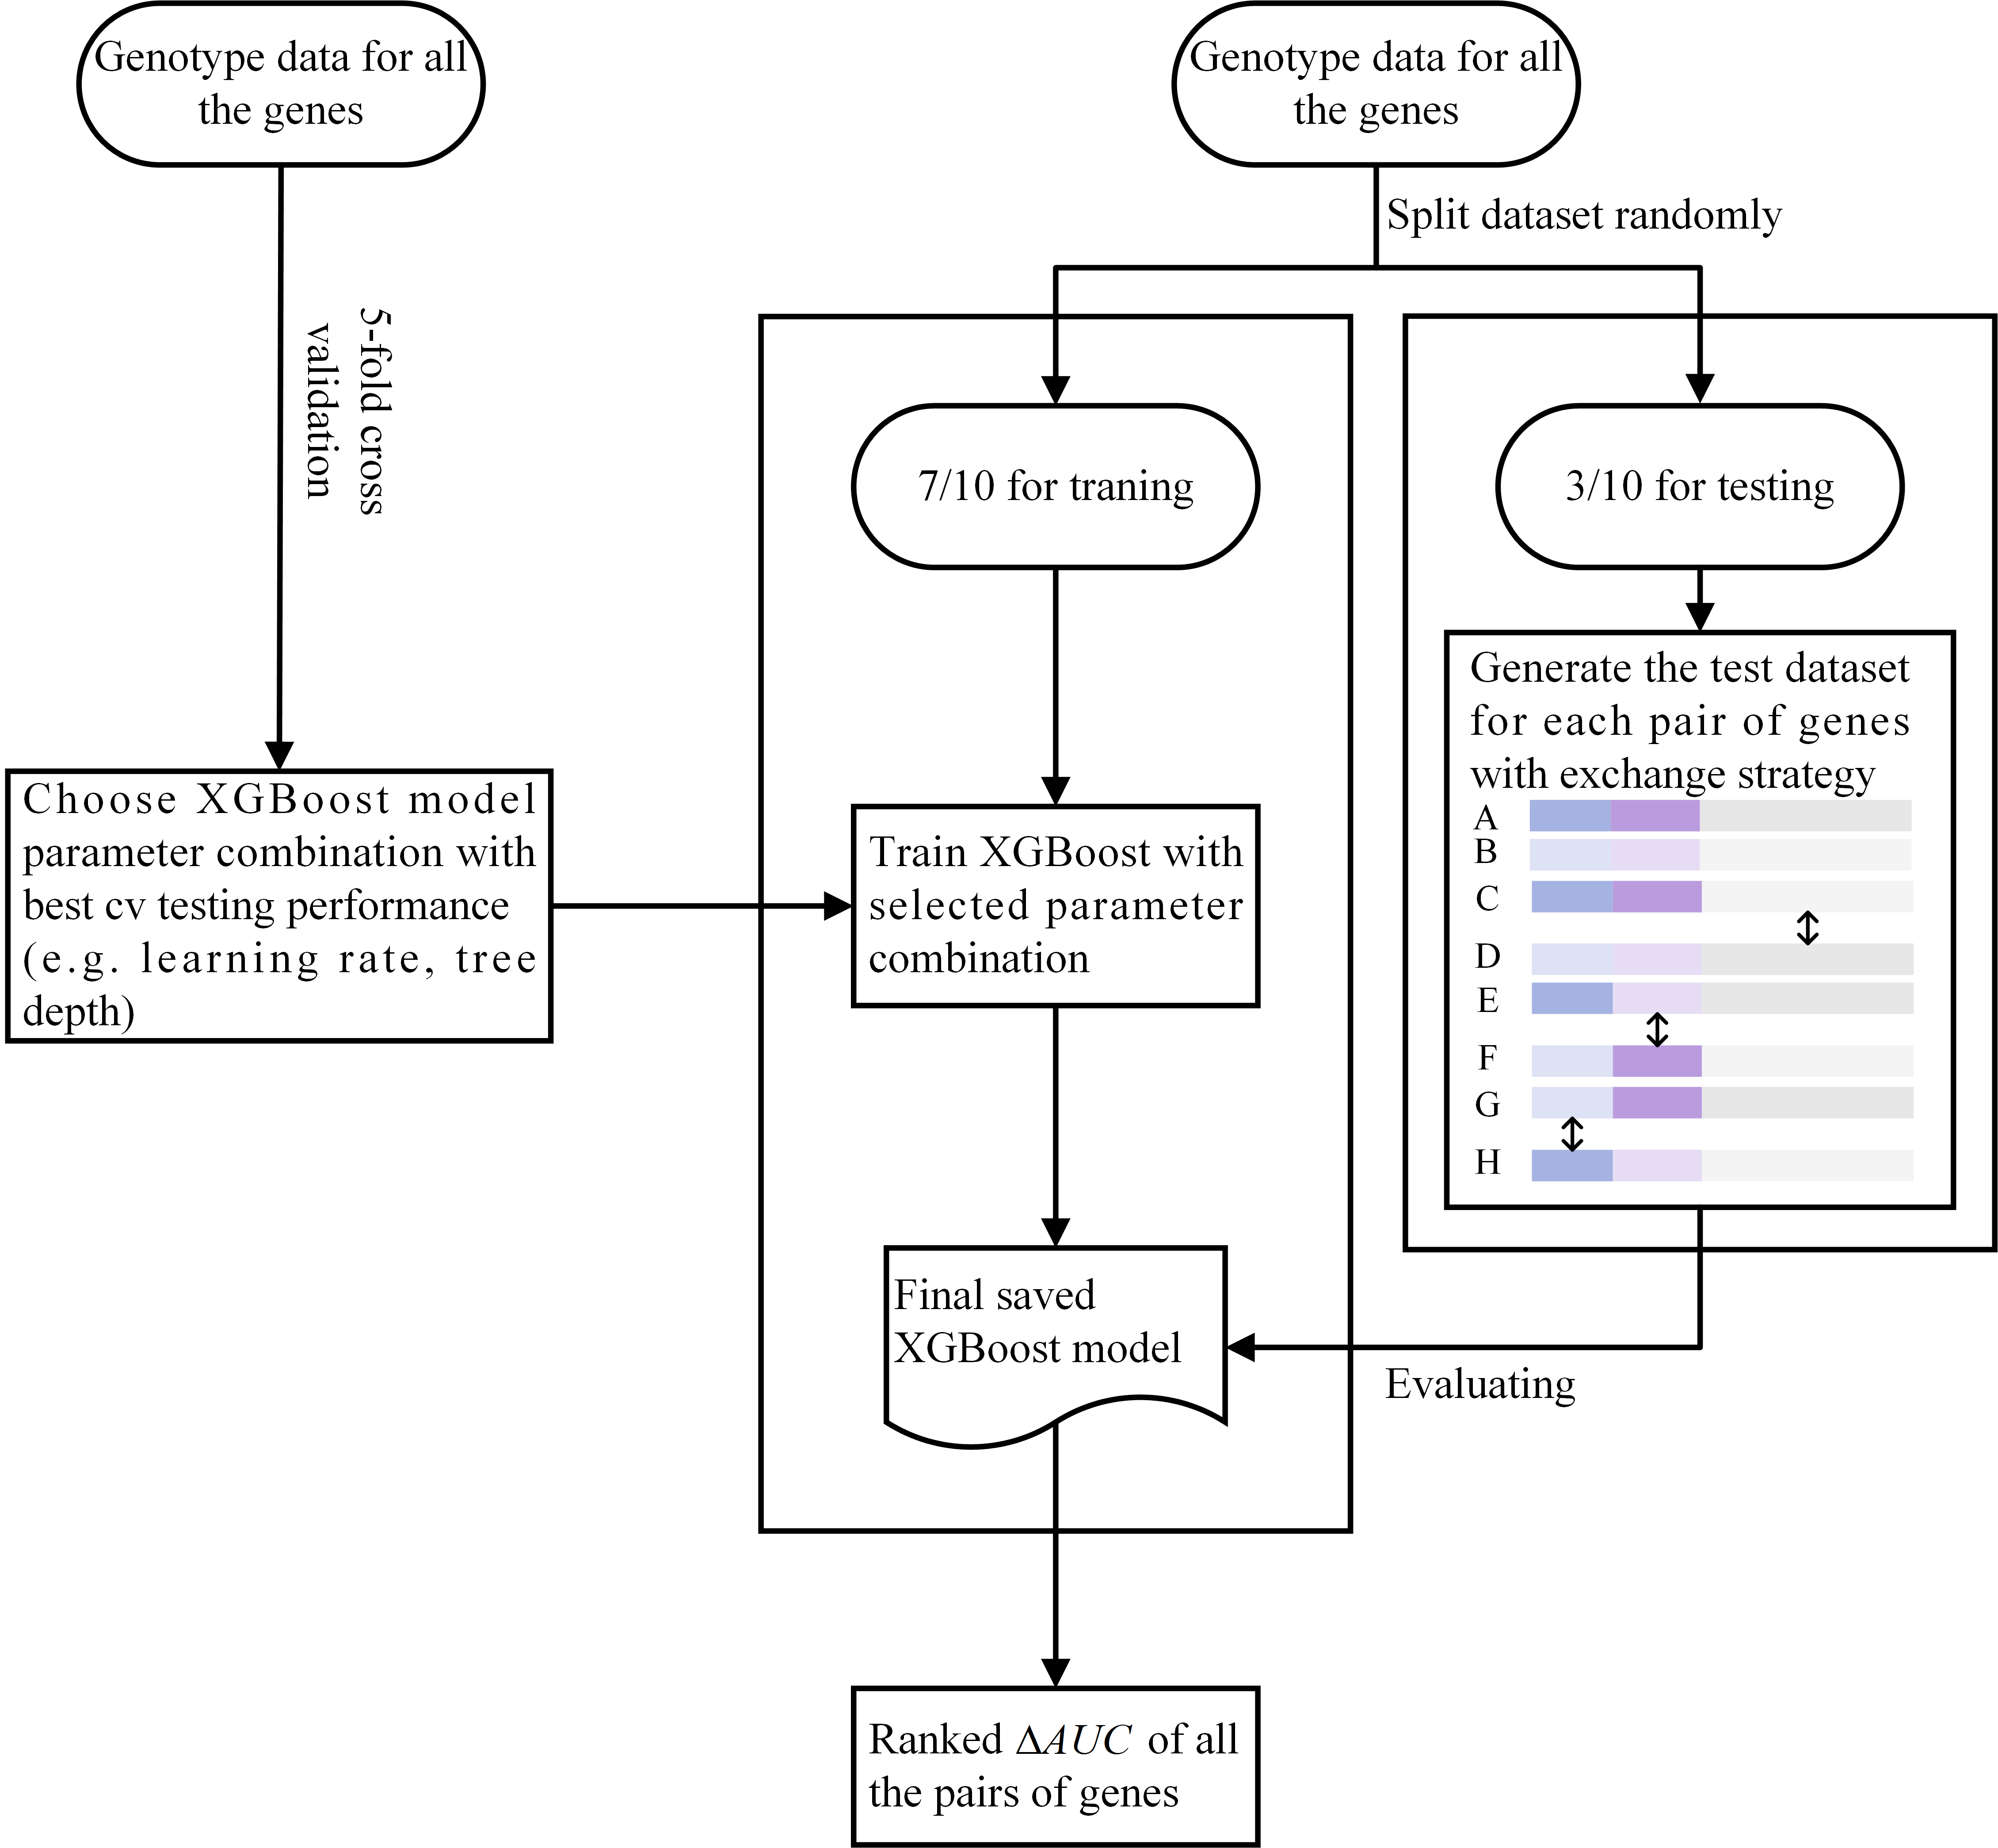
\includegraphics[scale=0.6]{framework_0116.png}
    \end{center}
\caption{\label{det}The framework of geXGB}
\end{figure}

\subsubsection{Overview of XGBoost}

XGBoost \cite{9} is a scalable supervised machine learning system based on tree boosting, and recently has been dominating applied machine learning as well as in Kaggle competitions. It is an algorithm which improves GBDT for speed with the same performance. In this section, we use the standard Machine Learning notation and let $x_i$ be features and $y$ be a binary random variable which we attempt to predict.

\paragraph{Ensemble of CARTs}
In this ensemble model, the base classifier is CART (Classifying And Regression Tree), which is similar to decision trees, but on each leaf, instead of a classification, a real-valued score is assigned. This makes ensemble training easier and may also provide more information beyond classification.\\

\noindent Let $\mathcal{F}$ be the space of functions that can be represented by CARTs, the ensemble predictor is $\hat{y}=\sum_k f_k, f_k\in\mathcal{F}$. In our case we interpret it as in logistic regression, namely
\begin{equation}
p(y=1|x)={1\over 1+e^{-\hat{y}(x)}}
\end{equation}

\noindent Hence, the learning objective is
\begin{equation}
obj=\sum_i(l(y_i,\hat{y}(x_i))+\sum_k\Omega(f_k)
\end{equation}
Where $l(y,\hat{y})=y\log(1+e^{-\hat{y}})+(1-y)\log(1+e^{\hat{y}})$ is the logistic regression loss function, and $\Omega(f_k)$ is the regularizer.

\paragraph{Gradient Boosting}
It is not feasible to train all the trees in the ensemble together at once because it is hard to calculate the gradient as which is needed in traditional optimization methods. Instead, XGBoost use an additive training strategy: fix the trees have already learned, add new trees one at a time. Let $\hat{y}^{(t)}$ be the predictor at iteration $t$, then
\begin{equation}
\hat{y}^{(0)}=0
\end{equation}
\begin{equation}
\hat{y}^{(t)}=\hat{y}^{(t-1)}+f_t
\end{equation}
Where $f_t\in\mathcal{F}$ optimizes the following target function, which is obtained by the Taylor expansion of the lost function for logistic regression to the second order.
\begin{equation}
obj^t=\sum_i\left(g_i(\hat{y}^{(t-1)}(x_i))f_t(x_i)+{h_i^2(\hat{y}^{(t-1)}(x_i))\over 2}\cdot f_t^2(x_i)\right)+\Omega(f_i)
\end{equation}
Here $g_i(\hat{y})={d\over d\hat{y}}l(y_i,\hat{y})$, $h_i(\hat{y})={d\over d\hat{y}}l(y_i,\hat{y})$.

\paragraph{Regularizer and Training strategy for CARTs}

For any $f\in\mathcal{F}$ , let $T$ be the number of leaves in the tree representing $f$ , $w_1,\dots, w_T$ be the scores on
the leaves. Then the regularizer used in XGBoost is
\begin{equation}
\Omega(f)=\gamma T+{1\over 2}\lambda\sum_j w_j^2
\end{equation}
The purpose of the second term is that it can smoothen the leaf scores.\\

\noindent To optimize $f_t$, firstly note that given a tree structure, $obj^t$ is a quadratic function of the scores $w_j$,
and the minimum of $obj^t$ as well as the $w_j$ that minimizes $obj^t$ can be easily calculated given the tree structure. Now the tree can be constructed by a greedy algorithm in which one starts with a tree with
one single node, and repeatedly split its leaves in a way that maximizes the decrease in $obj^t$ in each step.
\subsubsection{Evaluating and Ranking}

Our approach for gene-based gene-gene interaction detection is based on evaluating the extend a model trained with XGBoost (c.f. section 2.2) deviate from the ``product form'' in Equation (2). Our interaction estimation
technique is based on the following observation: if Equation (2) is satisfied for $X_g, X_g'$, and let $\mathcal{P}(X_g,X_g',X_\urcorner g,g'):=P(y=1|X_g,X_g',X_\urcorner g,g')$, $X_\urcorner g,g'$ be the vector consisting of genotypes that are in neither $X_g$ nor $X_{g'}$, then, for two samples $(X^A)$, $(X^B)$, we have
\begin{equation*}
\mathcal{P}(X^A_g,X^A_{g'},X^A_{\urcorner g,g'})\mathcal{P}(X^B_g,X^B_{g'},X^B_{\urcorner g,g'})\mathcal{P}(X^A_g,X^A_{g'},X^B_{\urcorner g,g'})\mathcal{P}(X^B_g,X^B_{g'},X^A_{\urcorner g,g'})
\end{equation*}
\begin{equation}=\mathcal{P}(X^A_g,X^B_{g'},X^A_{\urcorner g,g'})\mathcal{P}(X^B_g,X^A_{g'},X^B_{\urcorner g,g'})\mathcal{P}(X^A_g,X^B_{g'},X^B_{\urcorner g,g'})\mathcal{P}(X^B_g,X^A_{g'},X^A_{\urcorner g,g'})
\end{equation}
To verify that, note that if $\mathcal{P}(X_g,X_{g'},X_\urcorner g,g')=F_1(X_g, X_\urcorner g,g')*F_2(X_{g'},X_\urcorner g,g')$, then the left-hand-side of equation (9) above becomes:
\begin{equation*}
F_1(X^A_g,X^A_{\urcorner g,g'})F_2(X^A_{g'},X^A_{\urcorner g,g'})F_1(X^B_g,X^B_{\urcorner g,g'})F_2(X^B_{g'},X^B_{\urcorner g,g'})
\end{equation*}
\begin{equation*}
F_1(X^A_g,X^B_{\urcorner g,g'})F_2(X^A_{g'},X^B_{\urcorner g,g'})F_1(X^B_g,X^A_{\urcorner g,g'})F_2(X^B_{g'},X^A_{\urcorner g,g'})
\end{equation*}

\noindent while the right-hand-side becomes:
\begin{equation*}
F_1(X^A_g,X^A_{\urcorner g,g'})F_2(X^B_{g'},X^A_{\urcorner g,g'})F_1(X^B_g,X^B_{\urcorner g,g'})F_2(X^A_{g'},X^B_{\urcorner g,g'})
\end{equation*}
\begin{equation*}
F_1(X^A_g,X^B_{\urcorner g,g'})F_2(X^B_{g'},X^B_{\urcorner g,g'})F_1(X^B_g,X^A_{\urcorner g,g'})F_2(X^A_{g'},X^A_{\urcorner g,g'})
\end{equation*}


\noindent It is evident that these two are the same.\\

\noindent This observation is motivated by the well-known fact that a function $f(X,Y)$ is of the form $f(X,Y)=u(X)v(Y)$ if and only if for any $a,b,c,d$, $f(a,b)f(c,d)=f(a,d)f(c,b)$.\\

\noindent As the function $\mathcal{P}$ is unknown, we use the predicted probability of XGBoost as an estimator of it, and the extent of deviation from the ``product form'' is measured by the estimated difference between the left hand side and the right hand side of Equation (9). We want the distribution of the samples tested to be close to the samples we used to train the model to minimize error caused by interpolation. On the other hand, we don't want them to be completely identical because the learned probability may ill-behave at those places (c.f. \cite{13}). Hence, we randomly split the available sample set into two, using the 7/10 of the samples to train our model with the selected model parameters and the rest 3/10 to generate the test dataset for evaluating equation (9).The process of using exchange strategy to get the test dataset was shown in Figure 2.\\

\begin{figure}[H]
    \begin{center}
       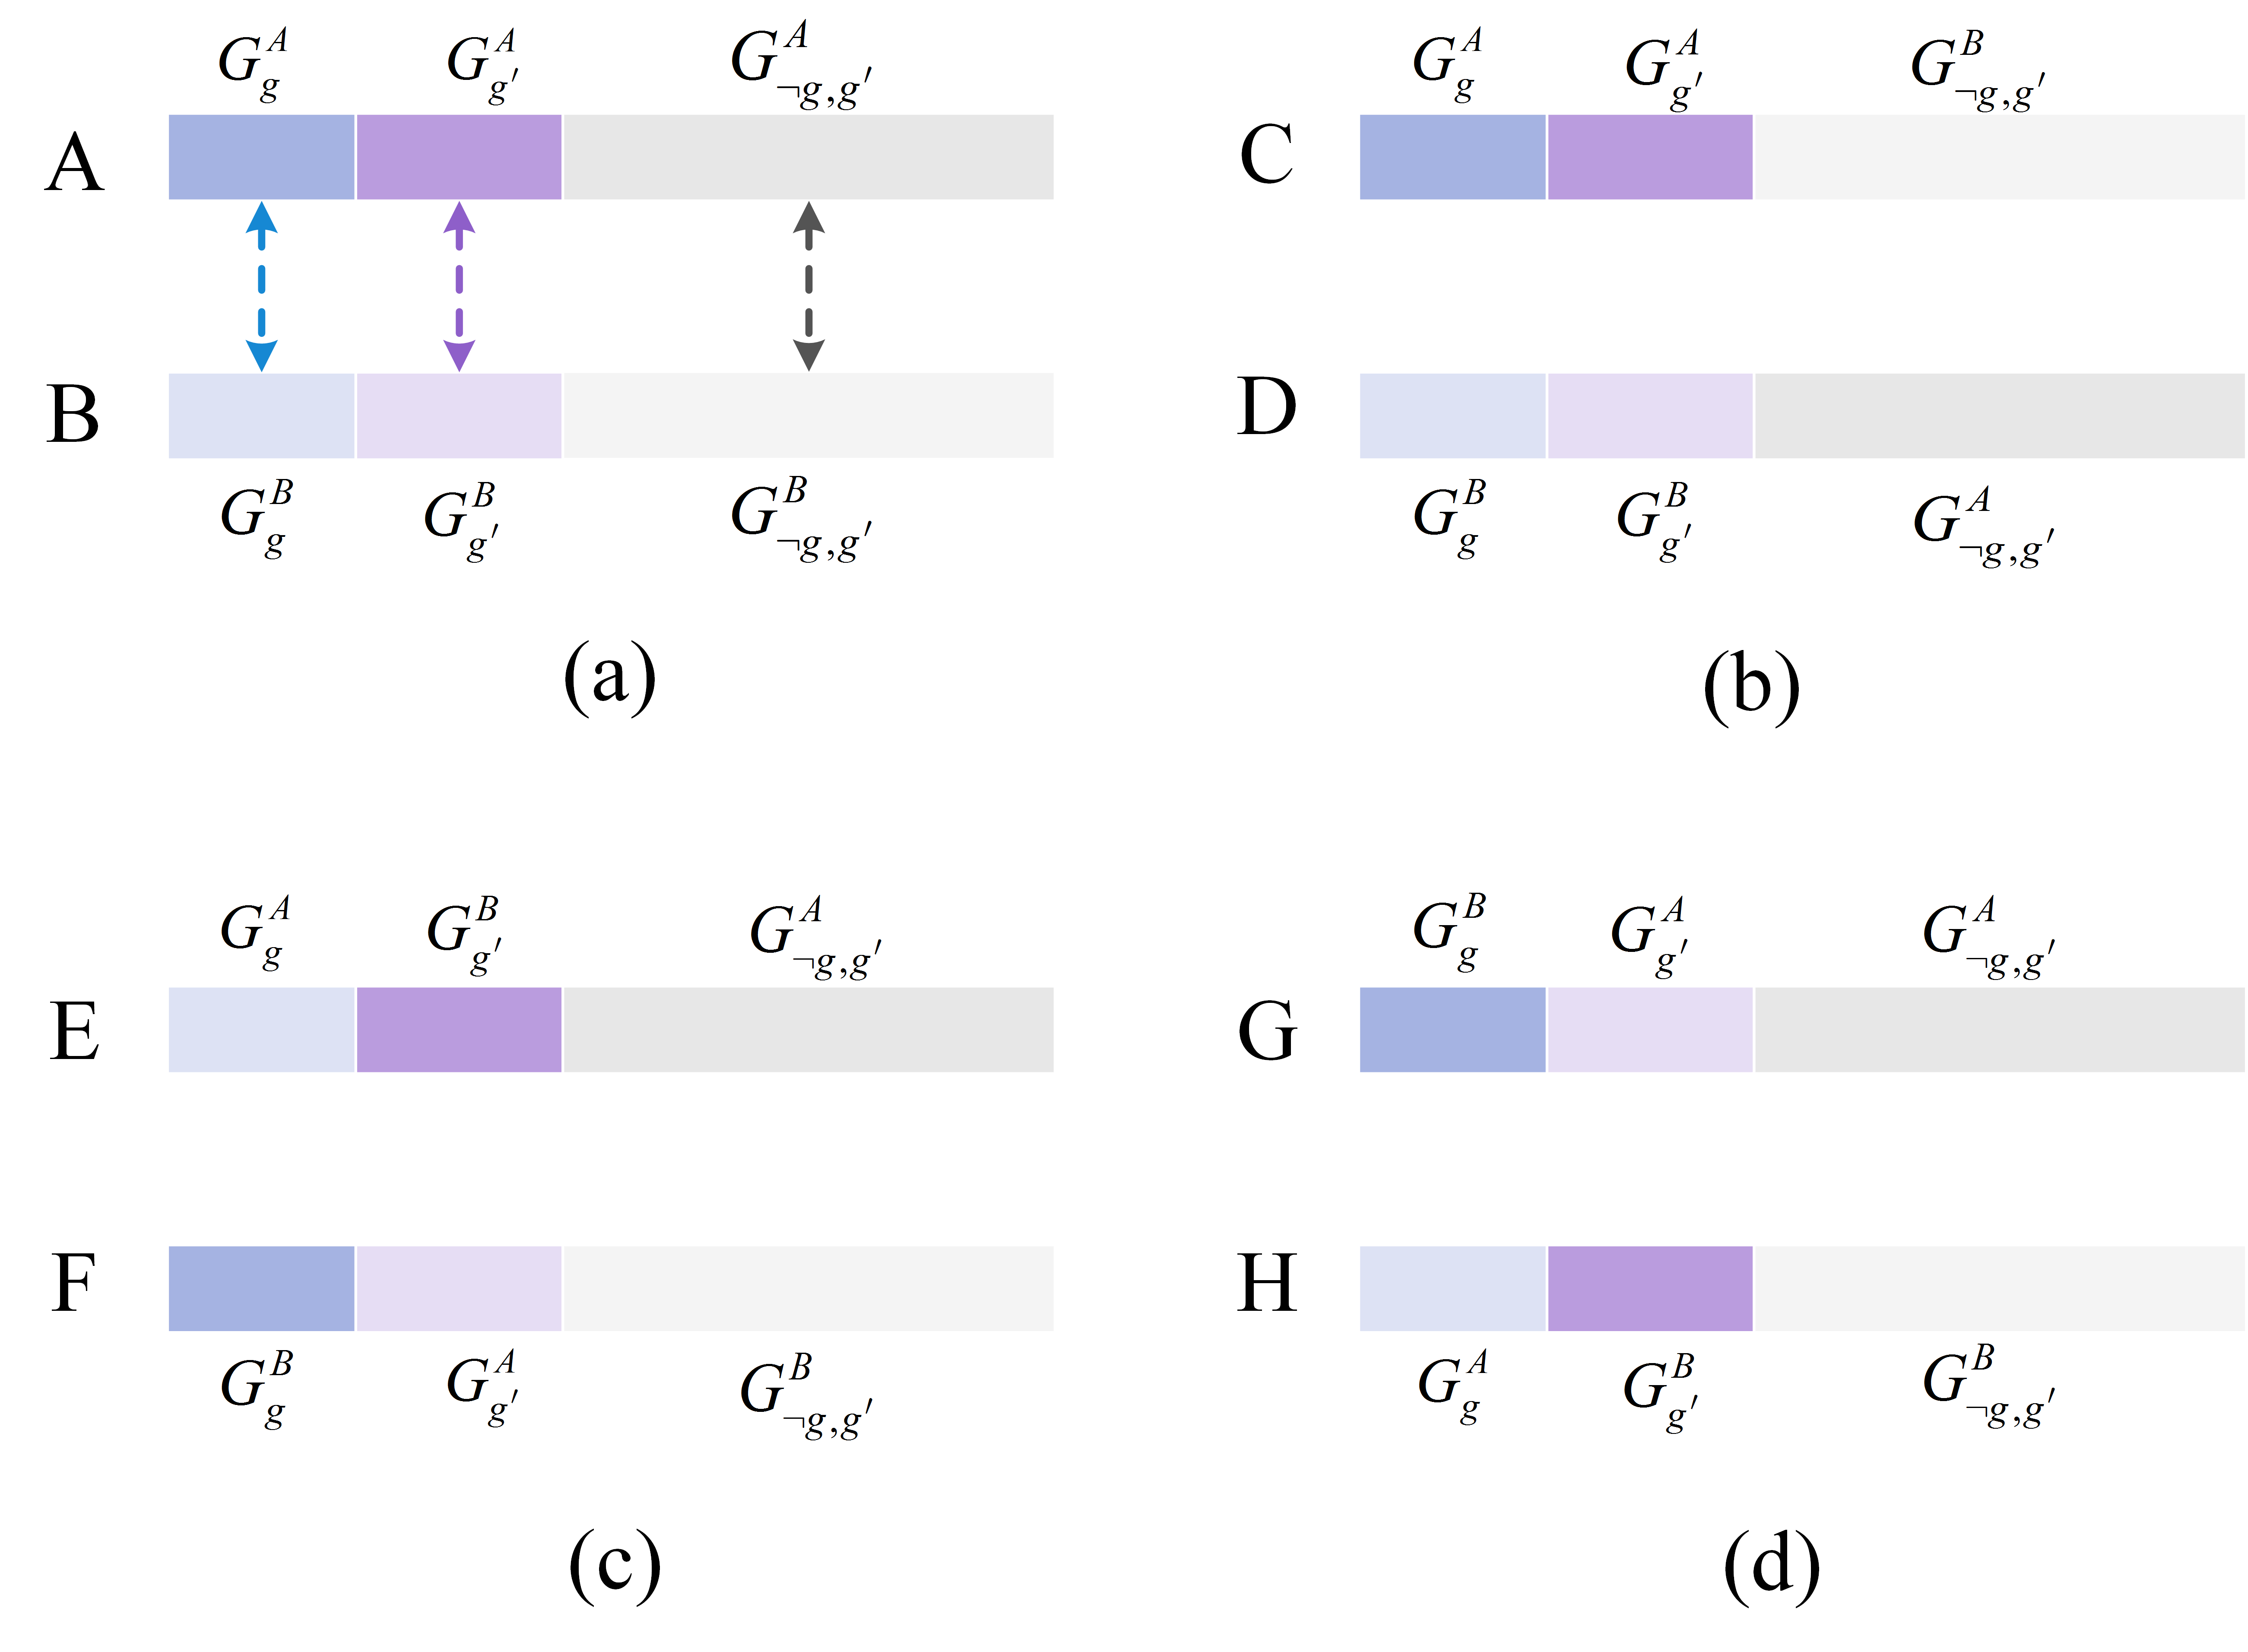
\includegraphics[scale=0.6]{exchange.png}
    \end{center}
\caption{\label{det}{\bf Illustration of exchange strategy of getting the test dataset:} (a) $A$ and $B$ are the two original samples from the test dataset, by exchanging the corresponding parts of $A$ and $B$ according to the rules indicated by the arrows, we obtain sets of genotypes $C,D,E,F,G,H$. (b) Exchange the genotypes in $A$ and $B$ in all genes except for the $g$-th and the $g'$-th, resulting in $C$ and $D$. (c)  Exchange the genotypes of the $g'$-th gene in $A$ and $B$, resulting in $E$ and $F$. (d) Exchange the genotypes of the $g$-th gene in $A$ and $B$, resulting in $G$ and $H$.}
\end{figure}

\noindent We obtain $C, D, E, F, G$ and $H$ according to Figure 2, then we calculated the absolute difference called $\Delta inter$ between the product of predicted probabilities of $A,B,C,D$ and $E,F,G,H$ for each pairs of genes. $\Delta inter$ can be treated as an indicator of the strength of gene-gene interaction that we ranked $\Delta inter$ for all the gene pairs and return the potential gene pairs that may interact.\\

\noindent Hence, with the considerations above, we propose our ranking algorithm as follows:

\begin{algorithm}[H]
\SetAlgoLined
\SetKwInOut{Input}{input}
\SetKwInOut{Output}{output}
\Input{genotype dataset $S=\{(x_1,y_1),(x_2,y_2)\dots (x_n,y_n)\}, x_i\in \mathbb\{0,1,2\}^{(m_1,\dots m_G)}, y_i\in \{0,1\} $; gene list file with position information for the $G$ genes; buffer region size.}
\Output{A list of all pairs of genes sorted by $\Delta inter$.}
Train XGBoost model, using grid search to find the proper parameter combination of the XGBoost, using 5-fold cross validation for each parameter combination and select the best parameter combination that gives the best average predictive performance.\\
\For{$i=1,\dots N$}{
Divide dataset $S$ randomly into a training set $S_{train}$ with 7/10 samples and a testing set $S_{test}$ with the rest.\\
XGBoostModel = trainXGBoost($S_{train}$, parameter combination)\\
Sample the testing dataset to obtain two sets of genotype data $A=\{{X^A}^i\}$ and $B=\{{X^B}^i\}$ of equal size.\\
\For{$1\leq g<g'\leq G$}{
Getting the $C=\{{X^C}^i\}$,$D=\{{X^D}^i\}$,$E=\{{X^E}^i\}$,$F=\{{X^F}^i\}$,$G=\{{X^G}^i\}$,$H=\{{X^H}^i\}$ according to the process shown in Figure2.

 $\Delta inter_{g,g'}=\sum_i(Predict(XGBoostModel, {X^A}^i)Predict(XGBoostModel, {X^B}^i)$\\
 $Predict(XGBoostModel, {X^C}^i)Predict(XGBoostModel, {X^D}^i)-$\\
 $Predict(XGBoostModel, {X^E}^i)Predict(XGBoostModel, {X^F}^i)$\\
 $Predict(XGBoostModel, {X^G}^i)Predict(XGBoostModel, {X^H}^i))$
}
}
Return $C^2_G$ pairs of genes sorted by the total $\Delta inter_{g,g'}$ in all $N$-iterations in decreasing order.
 \caption{geXGB}
\end{algorithm}

Because the first step is time consuming, in the simulated study, we did model selection for only one sample set and used the resulted parameters for the entire experiment.


% \subsubsection{Interpretation of the algorithm}

% Let $F(X_1,X_2)=P(y=1|X_1,X_2)$, and suppose the machine learning algorithm can capture $F$ perfectly. Then, the expected ROC after the permutation of the second type is
% \begin{equation}
% \left(\sum_{F(a,b)>p}P(X_1=a,X_2=b|Y=0),1-\sum_{F(a,b)<p}P(X_1=a,X_2=b|Y=1)\right)
% \end{equation}
% while the expected ROC of the permutation of the first type is:
% \begin{equation}
% \left(\sum_{F(a,b)>p}P(X_1=a|Y=0)P(X_2=b|Y=0),1-\sum_{F(a,b)<p}P(X_1=a|Y=1)P(X_2=b|Y=1)\right)
% \end{equation}

% Hence, the expected $\Delta AUC$ is
% \begin{align*}
% &\int_0^1\left(1-\sum_{F(a,b)<p}P(X_1=a,X_2=b|Y=1)\right)\\
% & d\left(\sum_{F(a,b)>p}P(X_1=a,X_2=b|Y=0)\right)-\\
% &\int_0^1 \left(1-\sum_{F(a,b)<p}P(X_1=a|Y=1)P(X_2=b|Y=1)\right)\\
% & d\left(\sum_{F(a,b)>p}P(X_1=a|Y=0)P(X_2=b|Y=0)\right)
% \end{align*}

% In particular, the AUCs are the same if $X_1$ and $X_2$ are conditionally independent with regards to $Y$.


\subsection{Simulation study}

The goal of this simulation study is to evaluate the performance of geXGB procedure for gene-gene interaction detection. All simulated datasets were set to have 50 SNPs. Among them 2 SNPs were functional and the remaining 48 SNPs were non-functional. The 50 SNPs formed 5 genes, each had 10 SNPs. The 2 functional SNPs were put into the first and second gene, and the performance is measured by how likely our algorithm can rank the two interacting genes as the most significant. We chose the publicly available tool GAMETES \cite{11} to generate the simulated genotype data. This tool is designed to generate epistasis models that we refer to as pure and strict. Purely and strictly epistasis models constitute the most difficult type of disease association model to detect, as such associations may be observed only if all n-loci are included in the disease model. This requirement makes these types of models an attractive gold standard for simulation studies of complex multi-locus effects. \\

\noindent In this simulation study, to test the effects of heritability (which measures the strength of correlation between genotype and phenotype) and sample size, we performed experiments under two different scenarios. In the first scenario, we tested two-locus epistasis models with five different heritabilities (0.01, 0.025, 0.05, 0.1 and 0.2) and two different minor allele frequencies (MAF, 0.2 and 0.4) with prevalence set to be 0.2 and sample size to be 3000. Ten models for each of the 10 heritability-allele frequency combinations were generated, so that we had 100 models in total in accordance to Hardy-Weinberg proportions. For a specified genetic constrain combination, the 10 models were roughly sorted by ascending customized odds ratio (COR) using GAMETES and then were labeled by M1 to M10. COR is a metrics of detectability that is calculated directly from the genetic model. The higher it is, the easier it is to detect the gene-gene interaction. The penetrance tables were generated for these 100 models in the absence of main effect. One hundred replicated data sets were generated from each model with balanced cases and controls, resulting in 10000 data sets in total in this scenario. In the second scenario, we set heritability to be 0.025 and MAF to be 0.2 and 0.4, prevalence to be 0.2 with sample size 10000. Then, 100 data sets were generated by random sampling from this large dataset for each of the 5 sample sizes 1000, 2000, 3000, 4000 and 5000. In this scenario, we have 1000 datasets in total.\\

\subsection{Real data analysis}
To assess the capacity of geXGB to deal with real case-control phenotype, we investigated the susceptibility of a set of pairs of genes to Rheumatoid Arthritis (RA), a chronic autoimmune joint disease where persistent inflammation affects bone remodeling leading to progressive bone destruction. We used the WTCCC(2007) dataset, which were genotyped in the British population using the Affymetrix GeneChip 500k. Quality control was performed in PLINK\cite{42} with several steps. First we removed samples with reported sex that did not match the heterozygosity rates observed on chromosome X \cite{12}. We additionally filtered out SNPs with $>10\%$ missingness,  with a minor allele frequency (MAF) $<0.05$, or for which missingness was significantly correlated with
phenotype ($p<1\times 10^{-4}$). We further filter out SNPs that are not in Hardy-Weinberg equilibrium in controls, as well as filter out samples with $>10\%$ missing SNPs. After the QC steps, we have XX SNPs, XXX samples with XXX cases and XXX controls.\\

\noindent In this analysis, we aim to verify some gene-gene interaction in the RA pathway hsa05323 in KEGG pathway dataset\cite{43}. Genotyping coordinates are given in NCBI Build36/UCSC hg18 (National Center for Biotechnology Information, Bethesda, MD). There are 90 genes in the pathway. Since MHCII and V-ATPase are two protein combinations that lots of interactions are within themselves, so we only choose a representative gene for each protein combinations and exclude other genes. After that, we can mapping 48 genes based on Build36 annotation. For each gene, 10-kb buffer region is added to both the upstream and downstream of the defined gene location. To address the effects of possible confounding variables, gender was included as covariate in the analysis. Principal component analysis was conducted using GCTA\cite{44}, and top 10 PCs were also included as covariates to account for potential population stratification.\\

\subsection{Competitive methods}
The performance of our procedure geXGB was compared to three previously published methods: Kernel Canonical Correlation-based U-statistic analysis (KCCU)\cite{4, 5}, the gene-based information gain method (GBIGM)\cite{6} and A Gene-based Gene-Gene interaction test method (AGGrEGATOr)\cite{7}. We adapted them to the task of ranking, by ranking the gene pairs by their p-values in ascending order.

\section{Results}

\subsection{Results for the simulation study}

To evaluate the statistical power of our geXGB and other three competitive methods, under each heritability-MAF combination, we measure the performance of geXGB by the relative frequency that the method ranks the interacting gene pair as the top one among the 100 data sets. For all other methods, the number listed is the relative frequency for the single interacting pair to have the smallest p-value.\\

\begin{table}[H]\footnotesize
\centering
\caption{Results of the first scenario of the simulation study}
\begin{tabular}{|c|c|c|cccccccccc|}
 \hline
  MAF & Herita- & \backslashbox{}{Model} & M1 & M2 &M3 & M4 &M5 &M6 &M7&M8&M9&M10\\
  &bility&Method&&&&&&&&&&\\
  \hline
  0.2&0.01&geXGB&0.14&{\bf 0.17}&{\bf 0.58}&0.75&{\bf 0.48}&{\bf 0.38}&0.71&0.91&{\bf 0.93}&{\bf 0.49}\\
  \cline{3-13}
     &&AGGrEGATOr&0.12&0.14&0.12&{\bf 0.89}&0.12&0.1&{\bf 0.89}&{\bf 1}&0.88&0.34\\
  \cline{3-13}
     &&KCCU&{\bf 0.15}&0.09&0.09&0.29&0.14&0.1&0.43&0.62&0.52&0.13\\
  \cline{3-13}
      &&GBIGM&0.09&0.08&0.11&0.13&0.12&0.17&0.11&0.08&0.1&0.09\\
  \cline{2-13}
      &0.025&geXGB&0.98&{\bf 0.97}&{\bf 0.94}&{\bf 1}&{\bf 1}&{\bf 0.99}&{\bf 0.99}&{\bf 1}&{\bf 0.9}&{\bf 0.94}\\
  \cline{3-13}
     &&AGGrEGATOr&{\bf 1}&0.15&0.27&{\bf 1}&{\bf 1}&0.46&0.37&{\bf 1}&0.69&0.81\\
   \cline{3-13}
      &&KCCU&0.58&0.09&0.09&0.74&0.71&0.59&0.24&0.8&0.12&0.12\\
  \cline{3-13}
&&GBIGM&0.08&0.11&0.07&0.11&0.1&0.12&0.13&0.2&0.14&0.1\\
\cline{2-13}
      &0.05&geXGB&{\bf 1}&{\bf 1}&{\bf 1}&{\bf 1}&{\bf 1}&{\bf 1}&{\bf 1}&{\bf 1}&{\bf 1}&{\bf 1}\\
  \cline{3-13}
      &&AGGrEGATOr&0.09&0.09&0.59&0.89&0.98&0.99&{\bf 1}&{\bf 1}&{\bf 1}&{\bf 1}\\
  \cline{3-13}
      &&KCCU&0.13&0.1&0.57&0.65&0.71&0.8&0.84&0.85&0.84&0.77\\
  \cline{3-13}
&&GBIGM&0.18&0.16&0.08&0.22&0.23&0.12&0.17&0.19&0.12&0.12\\
\cline{2-13}
 &0.1&geXGB&{\bf 1}&{\bf 1}&{\bf 1}&{\bf 1}&{\bf 1}&{\bf 1}&{\bf 1}&{\bf 1}&{\bf 1}&{\bf 1}\\
\cline{3-13}
&&AGGrEGATOr&{\bf 1}&{\bf 1}&{\bf 1}&{\bf 1}&{\bf 1}&{\bf 1}&{\bf 1}&{\bf 1}&{\bf 1}&{\bf 1}\\
\cline{3-13}
&&KCCU&0.81&0.88&0.93&0.9&0.9&0.83&0.86&0.91&0.84&0.93\\
\cline{3-13}
&&GBIGM&0.15&0.14&0.14&0.23&0.19&0.17&0.16&0.16&0.15&0.19\\
\cline{2-13}
&0.2&geXGB&{\bf 1}&{\bf 1}&{\bf 1}&{\bf 1}&{\bf 1}&{\bf 1}&{\bf 1}&{\bf 1}&{\bf 1}&{\bf 1}\\
\cline{3-13}

&&AGGrEGATOr&{\bf 1}&{\bf 1}&{\bf 1}&{\bf 1}&{\bf 1}&{\bf 1}&{\bf 1}&{\bf 1}&{\bf 1}&{\bf 1}\\
\cline{3-13}
&&KCCU&0.89&0.91&0.97&0.94&0.95&0.92&0.89&0.97&0.94&0.97\\
\cline{3-13}
      &&GBIGM&0.19&0.21&0.31&0.18&0.29&0.23&0.22&0.21&0.23&0.22\\
  \hline
  0.4&0.01&geXGB&{\bf 0.9}&{\bf 0.74}&{\bf 0.82}&{\bf 0.82}&{\bf 0.83}&{\bf 0.96}&{\bf 0.96}&{\bf 0.66}&0.82&{\bf 0.89}\\
\cline{3-13}
&&AGGrEGATOr&0.71&0.73&0.09&0.1&0.77&{\bf 0.96}&0.94&0.17&{\bf 0.9}&0.81\\
\cline{3-13}
&&KCCU&0.34&0.34&0.05&0.08&0.4&0.29&0.77&0.16&0.73&0.61\\
\cline{3-13}
&&GBIGM&0.09&0.11&0.08&0.1&0.11&0.07&0.11&0.18&0.11&0.11\\
\cline{2-13}
      &0.025&geXGB&{\bf 1}&{\bf 1}&{\bf 1}&{\bf 1}&{\bf 1}&{\bf 1}&{\bf 1}&{\bf 1}&{\bf 1}&{\bf 1}\\
  \cline{3-13}
      &&AGGrEGATOr&0.99&{\bf 1}&0.56&0.12&0.06&0.26&0.91&0.51&0.12&{\bf 1}\\
  \cline{3-13}
      &&KCCU&0.58&{\bf 1}&0.24&0.08&0.06&0.11&0.24&0.32&0.12&{\bf 1}\\
  \cline{3-13}
&&GBIGM&0.15&0.1&0.12&0.14&0.08&0.09&0.11&0.08&0.05&0.08\\
\cline{2-13}
      &0.05&geXGB&{\bf 1}&{\bf 1}&{\bf 1}&{\bf 1}&{\bf 1}&{\bf 1}&{\bf 1}&{\bf 1}&{\bf 1}&{\bf 1}\\
  \cline{3-13}
      &&AGGrEGATOr&{\bf 1}&0.68&0.97&0.91&0.15&0.42&0.35&0.19&0.91&{\bf 1}\\
  \cline{3-13}
      &&KCCU&0.86&0.15&0.9&0.95&0.1&0.37&0.41&0.14&0.74&{\bf 1}\\
  \cline{3-13}
      &&GBIGM&0.11&0.07&0.12&0.09&0.13&0.1&0.08&0.08&0.13&0.16\\
  \cline{2-13}
      &0.1&geXGB&{\bf 1}&{\bf 1}&{\bf 1}&{\bf 1}&{\bf 1}&{\bf 1}&{\bf 1}&{\bf 1}&{\bf 1}&{\bf 1}\\
  \cline{3-13}
      &&AGGrEGATOr&0.98&0.06&{\bf 1}&0.96&{\bf 1}&{\bf 1}&{\bf 1}&{\bf 1}&{\bf 1}&{\bf 1}\\
  \cline{3-13}
      &&KCCU&0.62&0.17&{\bf 1}&0.95&{\bf 1}&{\bf 1}&{\bf 1}&{\bf 1}&{\bf 1}&{\bf 1}\\
  \cline{3-13}
      &&GBIGM&0.12&0.17&0.19&0.18&0.12&0.2&0.13&0.1&0.19&0.12\\
  \cline{2-13}
      &0.2&geXGB&{\bf 1}&{\bf 1}&{\bf 1}&{\bf 1}&{\bf 1}&{\bf 1}&{\bf 1}&{\bf 1}&{\bf 1}&{\bf 1}\\
  \cline{3-13}
      &&AGGrEGATOr&0.93&{\bf 1}&{\bf 1}&0.99&{\bf 1}&0.8&0.27&0.09&0.14&0.12\\
  \cline{3-13}
      &&KCCU&0.28&{\bf 1}&{\bf 1}&0.83&{\bf 1}&0.76&0.41&0.15&0.28&0.12\\
  \cline{3-13}
&&GBIGM&0.19&0.2&0.25&0.31&0.23&0.26&0.26&0.29&0.22&0.1\\


\hline

\end{tabular}
\end{table}

\begin{table}[H]\footnotesize
\centering
\caption{Average power in the first scenario}
\begin{tabular}{|c|cccc|cccc|}
  \hline
  MAF&&0.2&&&&0.4&&\\
  \hline
  \backslashbox{}{Methods}&geXGB&AGGrE&KCCU&GBIGM&geXGB&AGGrE&KCCU&GBIGM\\
  Heritability&&GATOr&&&&GATOr&&\\
  \hline
  0.01&0.554&0.46&0.256&0.108&0.84&0.618&0.377&0.107\\
\hline
  0.025&0.971&0.675&0.408&0.116&1&0.553&0.375&0.1\\
\hline
  0.05&1&0.763&0.626&0.159&1&0.658&0.562&0.107\\
\hline
  0.1&1&1&0.879&0.168&1&0.9&0.874&0.152\\
  \hline
  0.2&1&1&0.935&0.229&1&0.634&0.583&0.231\\
  \hline
\end{tabular}
\end{table}


\begin{table}[H]\footnotesize
\centering
\caption{Results of the second scenario}
\begin{tabular}{|c|c|c|c|c|c|}
  \hline
  Heritability&\backslashbox{Sample Size}{Method}&geXGB&AGGrGETOr&KCCU&
                                                                        GBIGM\\
  \hline
             &1000&0.67&0.15&0.11&0.2\\
  \cline{2-6}
              &2000&1&0.18&0.38&0.16\\
  \cline{2-6}
  0.2&3000&1&0.11&0.55&0.23\\
  \cline{2-6}
              &4000&1&0.31&0.76&0.21\\
  \cline{2-6}
              &5000&1&0.26&0.87&0.12\\
  \hline
              &1000&0.68&0.18&0.13&0\\
  \cline{2-6}
              &2000&0.97&0.16&0.11&0.04\\
  \cline{2-6}
  0.4&3000&1&0.35&0.2&0.11\\
  \cline{2-6}
              &4000&1&0.54&0.37&0.11\\
  \cline{2-6}
  &5000&1&0.65&0.58&0.05\\
  \hline
\end{tabular}
\end{table}

\noindent Table 1 shows the empirical statistical power of all methods on the simulated data sets of the first scenario. Table 2 shows the average statistical power of Table 1. Table 3 displays the average statistical power of all methods on the simulated data sets of the second scenario. Figure~\ref{det} is a boxplot summary of Table 1. Bold font shows the best performed method in each model under a given heritability-MAF combination. Notice that a larger value indicates better performance. On average, geXGB is the best performing algorithm in this comparison, it largely outperforms the other methods, but not for all the data sets: on some data sets it yields to AGGrEGATOr. However, its performance is remarkably consistent and is the top performer for most data sets. AGGrEGATOr can achieve the same performance when MAF is 0.2 and heritability is larger than 0.05, while geXGB gives much better performance under smaller heritability. When heritability is the smallest value, 0.01, geXGB outperforms in 6 models while AGGrEGATOr in 3 when MAF=0.2, and 9 v.s.2 when MAF=0.4. AGGrEGATOr has better average performance than KCCU. However, when it underperforms on a data set, its performance can be very low, even lower than KCCU, for instance in M7,M8,M9 of (h=0.2,MAF=0.4). The Figure~\ref{det} also shows that AGGrEGATOr has a large range of performance for the 10 models. But geXGB does not exhibit this poor behavior. \\

\noindent KCCU is able to detect the interaction of some simulated disease models in our study. Figure~\ref{avg} shows the relationship between heritability and the average performance. From it, we can see that KCCU has the similar performance pattern with AGGrEGATOr, although AGGrEGATOr is much more powerful in most of the simulated scenarios. GBIGM has little power in detecting this type of gene-gene interaction with only one causal pair. This result replicated Emily's \cite{7} result of simulation. \\

\noindent Considering the relationship between performance of geXGB and genetic constrains, as expected, power of all the simulation is affected greatly by heritability, i.e. the effect size of the interaction. With heritability going from 0.01 to 0.025, geXGB almost doubled its power for a given sample size of $n=3000$ with $MAF=0.2$. Other methods are also shown an steady upward trend (Table 1). It also depends on the minor allele frequencies (MAF) of the interacting SNPs, e.g. for the cases of h=0.01, the power of the different simulations ranges between 0.14-0.93 for $MAF=0.2$, while it ranges between 0.66-0.96 for $MAF=0.4$ (Table 1). The average power is 0.554 for $MAF=0.2$, which is much lower than 0.84 for $MAF=0.4$ (Table 2). Sample size of the data set has a considerable effect on power as well, geXGB, AGGrGETOr and KCCU have lower power estimated for $n=1000$ compared to $n=5000$ (Table 3).

\noindent Thus, our results demonstrate that geXGB is particularly efficient in detecting gene-gene interaction where one SNP pair is assumed to be causal by the purely and strictly epistasis without main effect. Compared to other methods, geXGB has the capacity to accurately identify a wider range of epistatic signals.

\begin{figure}[H]
    \begin{center}
       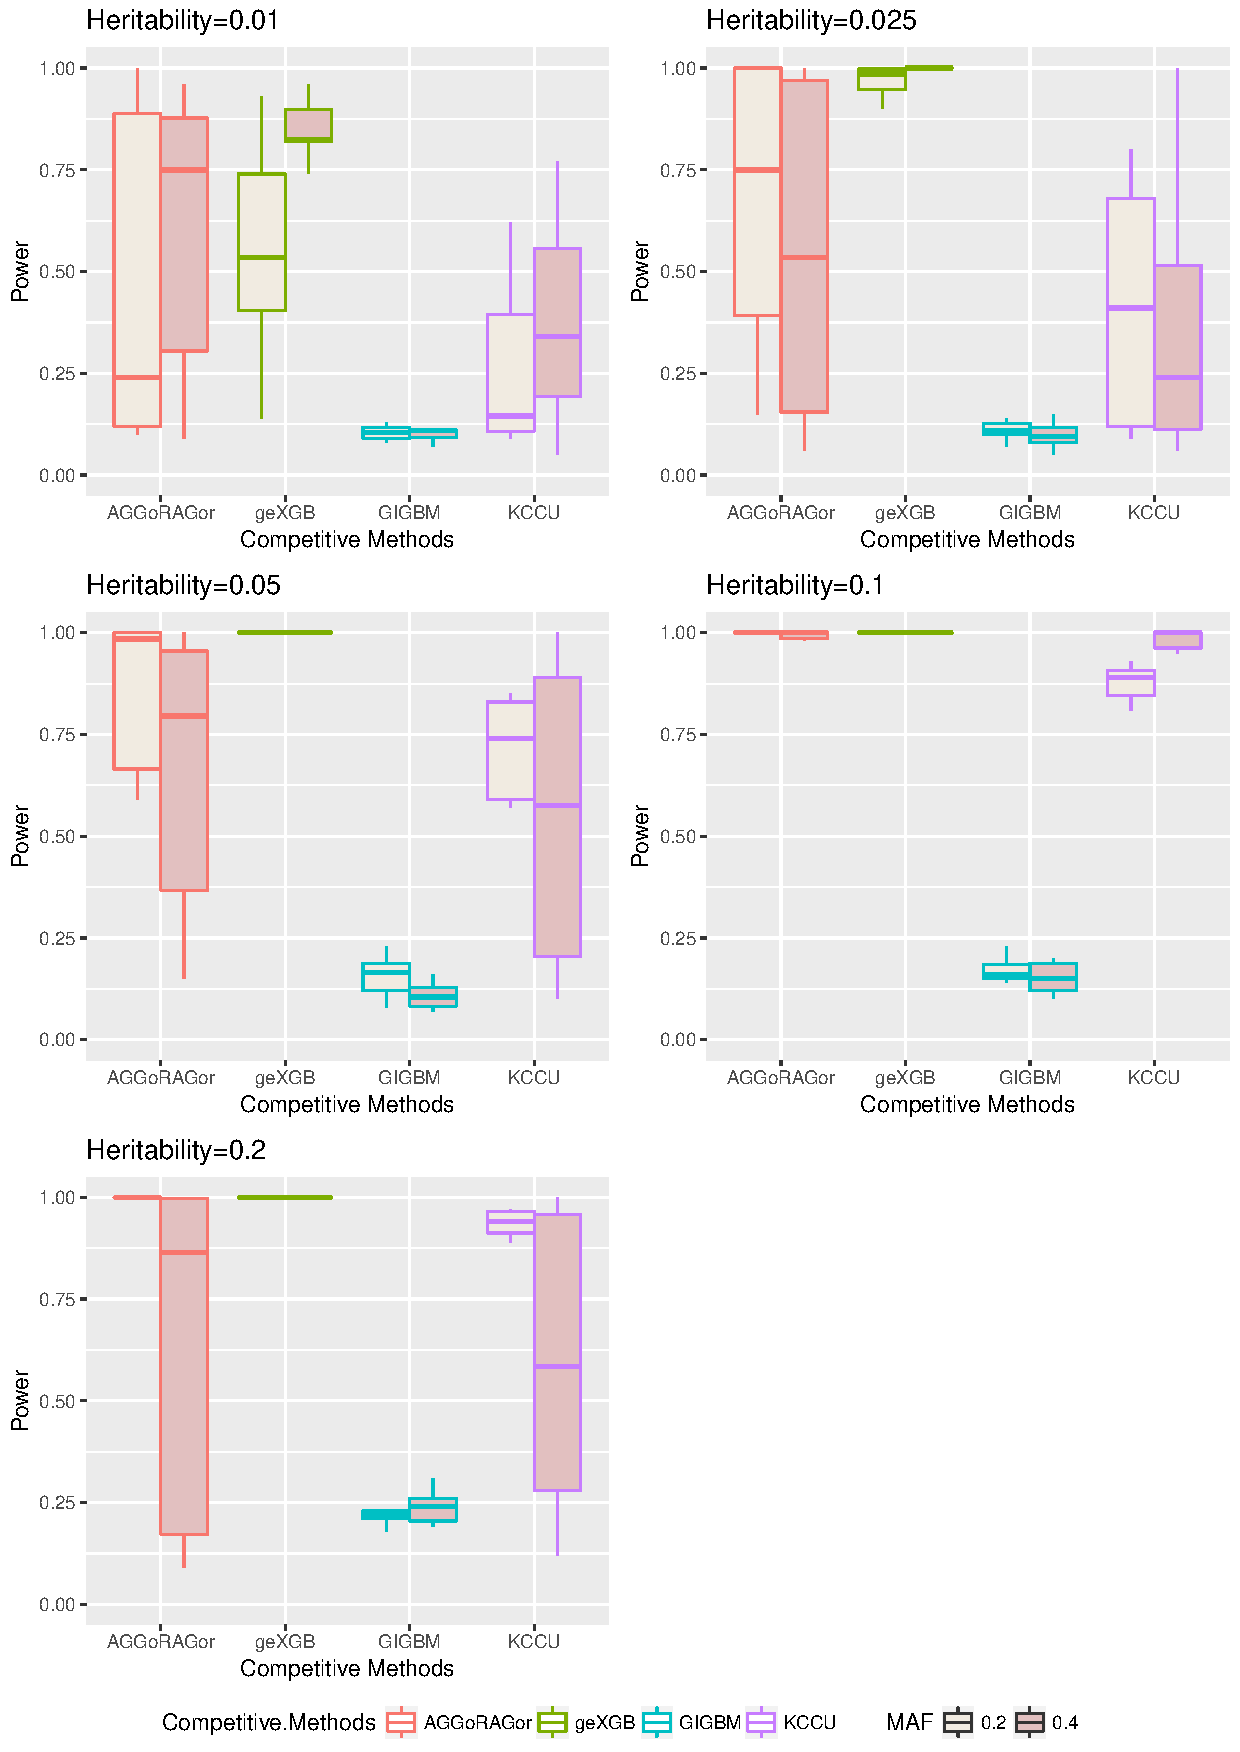
\includegraphics[scale=0.6]{boxplot10_simu.pdf}
    \end{center}
\caption{\label{det}Performance on the simulated datasets}
\end{figure}

\begin{figure}[H]
    \begin{center}
       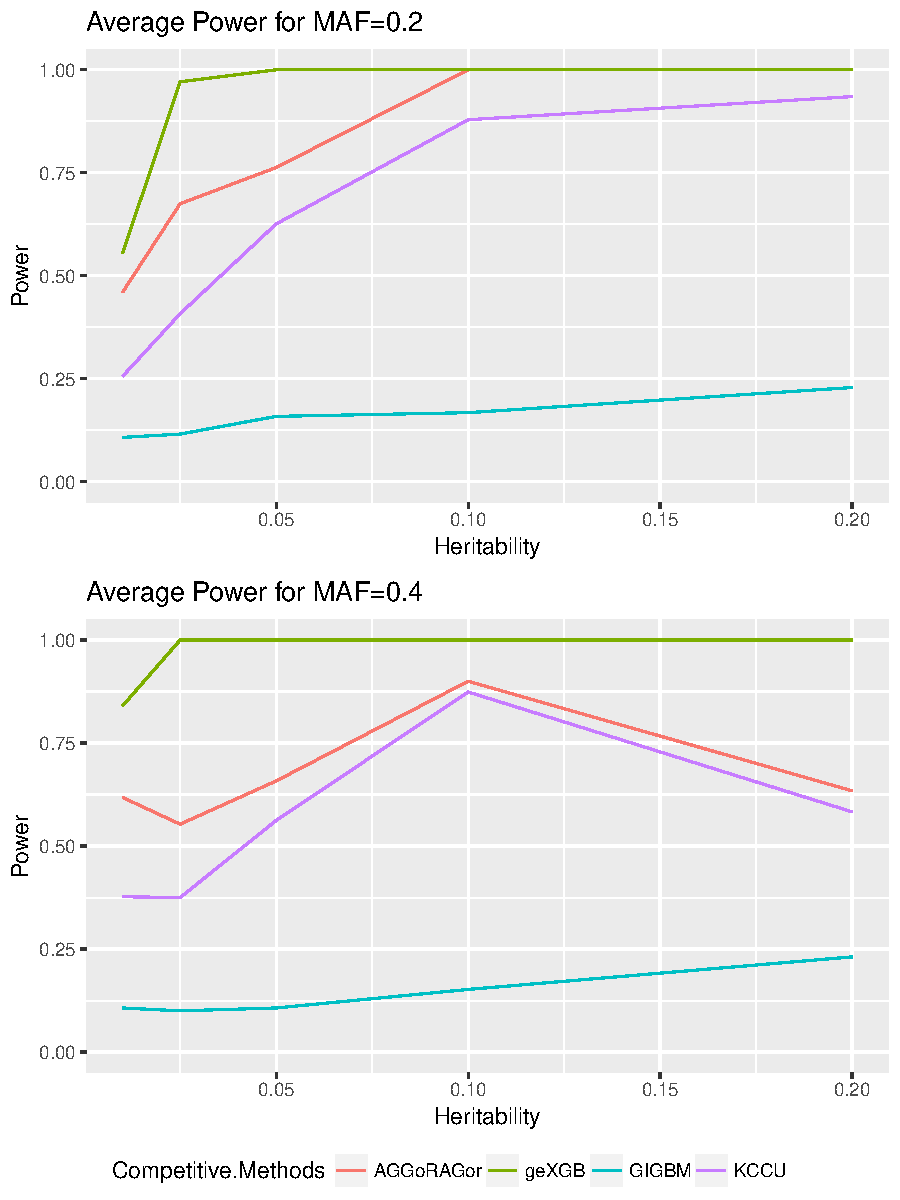
\includegraphics[scale=0.5]{average0204.pdf}
    \end{center}
\caption{\label{avg}Average performance on the simulated datasets}
\end{figure}


\subsection{Real data sets analysis}

For the Rheumatoid Arthritis(RA) study of the hsa05323 pathway, each unique gene pair was evaluated, resulting in $C_{48}^2=1128$ total pairs for 48 genes. We performed each of the methods 10 times to avoid any influence of random effects. With significance level $\alpha=0.01$ and multiple testing adjustment, for KCCU and GIGBM, we obtained around 43 and 65 significant GGIs, respectively. Among them, 30 and 65 have p-value equal to 0 hence we are unable to rank them in the order of significance. AGGrGETOr did not have any significant result. Following \cite{7}, after removing the multiple testing correction, AGGrGETOr got around 16 significant GGIs, which we rank by their p-values. As for geXGB, the $\Delta inter$ had a dramatic drop between the first and the second pair of genes, and a second drop happened around the seventh pair. Hence we chose the top 10 gene pairs obtained by geXGB and AGGrGETOr to analyze, constituting approximately $1\%$ of the total interactions. \\

\noindent The most significant interaction found by geXGB is Angiopoietin (Ang)1-Tie2. This interaction has already been verified. Synovial angiogenesis is a critical early event in RA, fostering pannus formation, persistent leukocyte infiltration, and lining layer hyperplasia, leading to cartilage and bone destruction\cite{14,15}. RA angiogenesis is driven and maintained by proangiogenic factors released from RA synovial tissue myeloid cells and fibroblasts, which include angiopoietin (Ang)1 and 2 \cite{16,17}. The endothelial cell(EC) specific factor Ang1 and Ang2 and their tyrosine kinase receptors Tie1 and Tie2 are critical in normal and pathological vascular development \cite{18}. Ang1, Ang2, Tie1, and Tie2 are upregulated in RA synovial tissues. Evidence suggests that the Ang/Tie2 signaling pathway mediates the proangiogenic effects of tumor necrosis factor alpha ($TNF-\alpha$), interleukin (IL)-6, and tolllike receptor (TLR)2 in RA \cite{17,19}. The seventh most significant pair found by AGGrEGATOr is interaction between RANKL and APRIL. It is shown that fibroblast-like synoviocytes (FLS) are among the principal effector cells in the pathogenesis of rheumatoid arthritis (RA), while APRIL increased RA FLS expression of RANKL \cite{20}. KCCU and GBIGM give a p-value of 0 to too many gene pairs that we are unable choose the top 10. \\

\begin{table}[H]\footnotesize
\centering
\caption{Summary of ranking results in the real dataset analysis}
\begin{tabular}{|c|c|cccc|}
  \hline
  Gene 1&Gene 2&&Ranking&&\\
  \cline{3-6}
  &&geXGB&AGGrGETOr&KCCU&GBIGM\\
  \hline
  Ang1&Tie2&1&1099&560&260\\
  \hline
  Tie2&Flt1&2&1108&685&460\\
  \hline
  Tie2&LFA1&3&1121&739&1035\\
  \hline
  MHCII&Ang1&4&1095&342&{\bf 70}\\
  \hline
  MHCII&Tie2&5&858&950&680\\
  \hline
  MCSF&Ang1&6&{\bf 3}&320&590\\
  \hline
  MCSF&Tie2&7&1033&485&495\\
  \hline
  Ang1&Flt1&8&1029&265&500\\
  \hline
  Tie2&RANK&9&1117&720&524\\
  \hline
  TGF-beta&Tie2&10&1037&745&580\\
  \hline
  CD86&CCL2&900&1&1066&650\\
  \hline
  TGF-beta&AP1&270&2&605&260\\
  \hline
  MCSF&Ang1&{\bf 6}&3&320&590\\
  \hline
  CD86&TLR4&650&4&{\bf 50}&565\\
  \hline
  CXCL1&RANKL&770&5&130&825\\
  \hline
  CCL20&TGF-beta&660&6&300&350\\
  \hline
  RANKL&APRIL&540&7&270&180\\
  \hline
  RANK&TGF-beta&340&8&875&{\bf 68}\\
  \hline
  IL23&LFA1&750&9&395&530\\
  \hline
  IL1&V-ATPase&1020&10&360&905\\
  \hline
\end{tabular}
\end{table}

\noindent Table 4 shows the RA results for four methods. We listed the top 10 of geXBG and AGGrEGATOr, respectively, and also give the ranking for these pairs in other three methods. Within the top 10 reuslts of geXBG and AGGrEGATOr, only one pair potential interaction between MCSF and Ang1 is captured by both methods. However, there is not yet direct evidence to show the interaction between MCSF and Ang1. Both geXBG and AGGrEGATOr have found a pair of meaningful interaction within a relative small number of results, however, there is almost no overlap between the results of the four methods.\\


\section{Discussion}


This study proposed geXGB, a new machine learning based procedure, to rank the significance of interaction at the gene level by applying the XGBoost algorithm to a GWAS sample and evaluate the deviation of result from a ``product form'' by an exchange strategy. We evaluated the power of geXGB to in ranking gene interaction of the pure and strict type through simulation study, and showed that it consistently outperforms prior methods on a wide range of disease models with different genetic constrain combinations.\\

\noindent In the geXGB procedure, due to the flexibility of XGBoost and the fact that the null hypothesis is that the classification probability is in a "product form", we avoided explicitly specifying the form of interactions between SNPs, hence rendered it more powerful compared to AGGrEGATOr or KCCU in some situation. Furthermore, our method can also easily incorporate the covariates matrix, hence take into account the corrections given by confounding information such as population stratification, sex and age, which is necessary for GWAS.\\

\noindent We applied the proposed methods to evaluate for gene-level interactions underlying Rheumatoid Arthritis (RA). We choose genes from a known RA pathway in KEGG to evaluate the performance of the method on real-life situation. The top pair interaction found by geXGB is between Ang1 and Tie2, which was proved to have an important role in synovial angiogenesis, an early event in RA. The seventh of AGGrEGATOr ranking result is also a meaningful pair interaction between APRIL and RANKL. Hence, when applying to real datasets, we suggest combining all the top results of the four methods as potential interactions since each method may capture a different aspect of the dataset.\\

\noindent Genome-wide implementation of geXGB is hardly feasible since the input of the model is all the candidate genes, too many unrelated genes may be harmful for the performance of the XGBoost model due to overfitting. To avoid the computational all the gene pairs, another strategy consists in using prior biological knowledge to reduce the number of genes need to be considered. Indeed, geXGB procedure can easily be used in a network based approach since it is widely assumed that protein-protein interaction network or pathway-based approach can be successfully combined to GWAS. Furthermore, the term ``gene'' refers to a collection of SNPs and can be any locus, even some non-function unit such as non-coding RNA. For all the reason we believe that the geXGB procedure can help detecting a part of the missing heritability. \\

From the real dataset experiment, we found that doing imputation to the dataset before applying the geXGB may give better performance, because genes with few SNPs could supply limited information that may be ignored by the ensemble trees, leading to the neglect of the interactions with these genes. As a result, it might be better to make sure that the genes have comparable number of SNPs. As for the LD structure, PLINK can be used to diminish the LD within a gene, while if two genes are correlated, the performance may be harmful since decision trees are by natrue immune to multi-collinearity though choose one of the correlated SNPs to split a node of a tree. This may underestimated a SNPs weight if there are several correlated SNPs. We recommend the use of geXGB when evaluating a group of unlinked genes or control the maximum of correlation does not exceed 0.1.\\

Although we have verified that geXGB procedure for detecting gene-gene interaction outperforms the previous methods on simulated pure and strict disease models and also be reliable on real dataset, there is still room for improvement our approach. The current version of our method do not provide a p-value to indicate how significant an interaction is. However, it can be modified to do so by adding ``fake genes'' which are genes whose genotype are obtained by permuting existing ones and does not provide any information on the phenotype, and counting the number of times pairs of ``real genes'' are picked in the ranking process. The procedure itself may also be modified to further exploring quantitative traits with replacing decision trees to regression trees, which is another important field in GWAS.


\section{Conflict of interest}

\section{Acknowledgements}

\begin{thebibliography}{99}
\bibitem{21}Hindorff L.A., et al., Potential etiologic and functional implications of genome-wide association loci for human diseases and traits. {\em Proc. Natl. Acad. Sci. U.S.A.}, 2009. 106:9362-9367.
\bibitem{22}MacArthur J., et al., The new NHGRI-EBI Catalog of published genome-wide association studies (GWAS Catalog). {\em Nucleic acids research}, 2016. p. gkw1133.
\bibitem{23}Carlborg O., et al., Epistasis: too often neglected in complex trait studies?. {\em Nature Reviews Genetics}, 2004. 5(8):618-625.
\bibitem{24}Cordell H.J., et al., {\em Detecting gene�Cgene interactions that underlie human diseases}. Nature Reviews Genetics, 2009. 10(6):392-404.
\bibitem{25}Moore J.H., et al., Bioinformatics challenges for genome-wide association studies. {\em Bioinformatics}, 2010. 26(4):445-455.
\bibitem{26}Manolio T.A., et al., Finding the missing heritability of complex diseases. {\em Nature}, 2009. 461(7265):747-753.
\bibitem{27}Moore J.H., et al., Epistasis and its implications for personal genetics. {\em The American Journal of Human Genetics}, 2009. 85(3):309-320.
\bibitem{28}Zuk O., et al., The mystery of missing heritability: Genetic interactions create phantom heritability. {\em Proceedings of the National Academy of Sciences}, 2012. 109(4):1193-1198.
\bibitem{29}Cordell H.J., et al., Epistasis: what it means, what it doesn't mean, and statistical methods to detect it in humans. {\em Human molecular genetics}, 2002. 11(20):2463-2468.
\bibitem{30}Marchini J., et al., Genome-wide strategies for detecting multiple loci that influence complex diseases. {\em Nature genetics}, 2005. 37(4):413-417.
\bibitem{31}Purcell S., et al., PLINK: a tool set for whole-genome association and population-based linkage analyses. {\em The American Journal of Human Genetics}, 2007. 81(3):559-575.
\bibitem{32}Emily M., IndOR: a new statistical procedure to test for SNP�CSNP epistasis in genome-wide association studies. {\em Statistics in medicine}, 2012. 31(21):2359-2373.
\bibitem{33}Jinying Z., et al., Test for interaction between two unlinked loci. {\em The American Journal of Human Genetics}, 2006. 79(5):831-845.
\bibitem{34}Xuesen W., et al., A novel statistic for genome-wide interaction analysis. {\em PLoS Genet}, 2010. 6(9):e1001131.
\bibitem{35}Ueki M., et al., Improved statistics for genome-wide interaction analysis. {\em PLoS Genet}, 2012. 8(4):e1002625.
\bibitem{36}Changzheng D., et al., Exploration of gene�Cgene interaction effects using entropy-based methods. {\em European Journal of Human Genetics}, 2008. 16(2):229-235.
\bibitem{37}Guolian K., et al., An entropy-based approach for testing genetic epistasis underlying complex diseases. {\em Journal of theoretical biology}, 2008. 250(2):362-374.
\bibitem{38}Ritchie M.D., et al., Power of multifactor dimensionality reduction for detecting gene-gene interactions in the presence of genotyping error, missing data, phenocopy, and genetic heterogeneity. {\em Genetic epidemiology}, 2003. 24(2):150-157.
\bibitem{39}Moore J.H., et al., Tuning ReliefF for genome-wide genetic analysis. {\em European Conference on Evolutionary Computation, Machine Learning and Data Mining in Bioinformatics}, 2007. Springer Berlin Heidelberg.
\bibitem{40}Cordell H.J., et al., Detecting gene�Cgene interactions that underlie human diseases. {\em Nature Reviews Genetics}, 2009. 10(6):392-404.
\bibitem{41}Xiang Z., et al., TEAM: efficient two-locus epistasis tests in human genome-wide association study. {\em Bioinformatics}, 2010. 26(12):i217-i227.
\bibitem{1}Wan, X., et al., BOOST: A fast approach to detecting gene-gene interactions in genome-wide case-control studies. {\em Am J Hum Genet}, 2010. 87(3):325-40.
\bibitem{2}Li, J., et al., Detecting gene-gene interactions using a permutation-based random forest method. {\em BioData Min}, 2016. 9:14.
\bibitem{45}Miaoxin L., et al., GATES: a rapid and powerful gene-based association test using extended Simes procedure. {\em The American Journal of Human Genetics}, 2011. 88(3):283-293.
\bibitem{46}Jimmy Z.L., et al., A versatile gene-based test for genome-wide association studies. {\em The American Journal of Human Genetics}, 2010. 87(1):139-145.
\bibitem{3}Peng, Q., J. Zhao, and F. Xue, A gene-based method for detecting gene-gene co-association in a case-control association study. {\em Eur J Hum Genet}, 2010. 18(5):582-7.
\bibitem{4}Yuan, Z., et al., Detection for gene-gene co-association via kernel canonical correlation analysis. {\em BMC Genet}, 2012. 13:83.
\bibitem{5}Larson, N.B., et al.,  Kernel canonical correlation analysis for assessing gene-gene interactions and application to ovarian cancer. {\em Eur J Hum Genet}, 2014. 22(1):126-31.
\bibitem{6}Li, J., et al., A gene-based information gain method for detecting gene-gene interactions in case-control studies. {\em Eur J Hum Genet}, 2015. 23(11):1566-72.
\bibitem{7}Emily, M., AGGrEGATOr: A Gene-based GEne-Gene interActTiOn test for case-control association studies. {\em Stat Appl Genet Mol Biol}, 2016. 15(avg2):151-71.
\bibitem{8}Ma, L., A.G. Clark, and A. Keinan,  Gene-based testing of interactions in association studies of quantitative traits. {\em PLoS Genet}, 2013. 9(2):e1003321.
\bibitem{9}Chen, T. and C. Guestrin. XGBoost: A Scalable Tree Boosting System. {\em Proceedings of the 22Nd ACM SIGKDD International Conference on Knowledge Discovery and Data Mining. ACM}. 2016. pp.785-894
\bibitem{13}Mentch, Lucas, and Giles Hooker, Formal hypothesis tests for additive structure in random forests. {\em Journal of Computational and Graphical Statistics}, 2016.
\bibitem{10}Greene, C.S., et al.,  Enabling personal genomics with an explicit test of epistasis. Pac Symp Biocomput, 2010:327-336.
\bibitem{42}Purcell S., et al., PLINK: a tool set for whole-genome association and population-based linkage analyses. {\em The American Journal of Human Genetics}, 2007. 81(3):559-575.
\bibitem{43}Kanehisa M., et al., KEGG: kyoto encyclopedia of genes and genomes. {\em Nucleic acids research}, 2000. 28(1):27-30.
\bibitem{44}Yang J., et al., GCTA: a tool for Genome-wide Complex Trait Analysis. {\em Am J Hum Genet}, 2011. 88(1):76-82.
\bibitem{11}Urbanowicz, R.J., et al., GAMETES: a fast, direct algorithm for generating pure, strict, epistatic models with random architectures. {\em BioData Min}, 2012. 5(1):16.
\bibitem{12}Laurie, C.C., et al., Quality control and quality assurance in genotypic data for genome-wide association studies. {\em Genet Epidemiol}, 2010. 34(6):591-602.
\bibitem{14}Elshabrawy H.A., et al., The pathogenic role of angiogenesis in rheumatoid arthritis. {\em Angiogenesis}, 2015. 18: 433-448.
\bibitem{15}Szekanecz Z., et al., Angiogenesis and vasculogenesis in rheumatoid arthritis. {\em Curr Opin Rheumatol}, 2010. 22: 299-306.
\bibitem{16}Nagashima M., et al., Role of vascular endothelial growth factor in angiogenesis of rheumatoid arthritis. {\em J. Rheumatol}, 1995. 22:1624-1630.
\bibitem{17}Kayakabe K., et al., Interleukin-6 promotes destabilized angiogenesis by modulating angiopoietin expression in rheumatoid arthritis. {\em Rheumatology (Oxford)}, 2012. 51:1571-1579.
\bibitem{18}Morisada T., et al., Angiopoietins and angiopoietin-like proteins in angiogenesis. {\em Endothelium}, 2006. 13:71-79.
\bibitem{19}Saber T., et al., Toll-like receptor 2 induced angiogenesis and invasion is mediated through the Tie2 signalling pathway in rheumatoid arthritis. {\em PLoS One}, 2011, 6:e23540.
\bibitem{20}Nagatani K., et al., Rheumatoid arthritis fibroblast-like synoviocytes express BCMA and are stimulated by APRIL. {\em Arthritis \& Rheumatism}, 2007. 56(11):3554-3563.


\end{thebibliography}



\end{document}
